%%%%%%%%%%%%%%%%%%%%%%%%%%%%%%%%%%%%%%
% LaTeX poster template
% Created by Nathaniel Johnston
% August 2009
% http://www.nathanieljohnston.com/2009/08/latex-poster-template/
%%%%%%%%%%%%%%%%%%%%%%%%%%%%%%%%%%%%%%

\documentclass[final]{beamer}
\usepackage[size = custom, width = 142, height = 91, scale=1.1]{beamerposter}
\usepackage{graphicx}			% allows us to import images
\graphicspath{ {/home/caleb/Link_to_HPV_Projects/smdm2017/Plots/} {C:/Users/caleb/HPV_Projects/smdm2017/Plots/}}
\usepackage[absolute,overlay]{textpos}
\usepackage[style = alphabetic,
    doi=false,
    isbn=false,
    url=false,
	maxbibnames = 5]{biblatex}
\addbibresource{hpv_bib_3_27.bib}
% remove notes: from http://tex.stackexchange.com/questions/208441/suppress-the-note-field-using-biblatex
\AtEveryBibitem{%
  \clearfield{note}%
}

\usepackage{setspace}
\singlespacing

% keep small bullets the same size
\setbeamerfont{itemize/enumerate subbody}{size = \large}

% for wrapping figures
\usepackage{wrapfig}

% use package csvsimple to read reduction table
\usepackage{csvsimple}
\usepackage{booktabs}
%-----------------------------------------------------------
% Define the column width and poster size
% To set effective sepwid, onecolwid and twocolwid values, first choose how many columns you want and how much separation you want between columns
% The separation I chose is 0.024 and I want 4 columns
% Then set onecolwid to be (1-(4+1)*0.024)/4 = 0.22
% Set twocolwid to be 2*onecolwid + sepwid = 0.464
%-----------------------------------------------------------

\newlength{\sepwid}
\newlength{\onecolwid}
\newlength{\twocolwid}
\newlength{\threecolwid}
\setlength{\paperwidth}{142.24 cm}
\setlength{\paperheight}{91.44 cm}
\setlength{\sepwid}{0.024\paperwidth}
\setlength{\onecolwid}{0.3\paperwidth}
\setlength{\twocolwid}{0.625\paperwidth}
\setlength{\threecolwid}{0.975\paperwidth}
\setlength{\topmargin}{-1in}
\usetheme{confposter}
\usepackage{exscale}
\usepackage{tikz}

%-----------------------------------------------------------
% The next part fixes a problem with figure numbering. Thanks Nishan!
% When including a figure in your poster, be sure that the commands are typed in the following order:
% \begin{figure}
% \includegraphics[...]{...}
% \caption{...}
% \end{figure}
% That is, put the \caption after the \includegraphics
%-----------------------------------------------------------

\usecaptiontemplate{
\large
\structure{\insertcaptionname~\insertcaptionnumber:}
\insertcaption}

%-----------------------------------------------------------
% Define colours (see beamerthemeconfposter.sty to change these colour definitions)
%-----------------------------------------------------------

\setbeamercolor{block title}{fg=ngreen,bg=white}
\setbeamercolor{block body}{fg=black,bg=white}
\setbeamercolor{block alerted title}{fg=white,bg=dblue!70}
\setbeamercolor{block alerted body}{fg=black,bg=dblue!10}
\setbeamercolor{block example title}{fg=white,bg=dgreen!70}
\setbeamercolor{block example body}{fg=black,bg=dgreen!10}



\makeatletter
%% Define a HUGE
\newcommand\HUGE{\@setfontsize\Huge{90}{80}}

\csvset{
  autotabularcenter/.style={
    file=#1,
    after head=\csv@pretable\begin{tabular}{|*{\csv@columncount}{c|}}\csv@tablehead,
    table head=\hline\csvlinetotablerow\\\hline,
    late after line=\\,
    table foot=\\\hline,
    late after last line=\csv@tablefoot\end{tabular}\csv@posttable,
    command=\csvlinetotablerow},
  autobooktabularcenter/.style={
    file=#1,
    after head=\csv@pretable\begin{tabular}{*{\csv@columncount}{c}}\csv@tablehead,
    table head=\csvlinetotablerow\\\midrule\midrule,
    late after line=\\,
    table foot=\\\bottomrule,
    late after last line=\csv@tablefoot\end{tabular}\csv@posttable,
    command=\csvlinetotablerow},
}
\makeatother
\newcommand{\csvautotabularcenter}[2][]{\csvloop{autotabularcenter={#2},#1}}
\newcommand{\csvautobooktabularcenter}[2][]{\csvloop{autobooktabularcenter={#2},#1}}



%-----------------------------------------------------------
% Name and authors of poster/paper/research
%-----------------------------------------------------------

\title{\HUGE{The Impact of Sexual Mixing By Age on Sexually Transmitted Infection Models}}
\author{Caleb Easterly, B.A., Fernando Alarid-Escudero, M.S., PhD., Eva Enns, PhD., \& Shalini Kulasingam, PhD.}
\institute{University of Minnesota}

%-----------------------------------------------------------
% Start the poster itself
%-----------------------------------------------------------

\begin{document}

		\addtobeamertemplate{headline}{}

\begin{frame}[t]
  \begin{columns}[t]	% the [t] option aligns the column's content at the top
    \begin{column}{\sepwid}\end{column}			% empty spacer column
    \begin{column}{1.1\onecolwid}
      \begin{block}{\textcolor{Black}{\Large{Background}}}
        \begin{itemize}
          \item Mathematical models of sexually transmitted infection (STI) dynamics are commonly used to evaluate interventions.
              For example, recently used to inform HPV vaccination policy recommendations.
          \item In STI models, a commonly used representation of sexual partner choice is the
            \textbf{assortative-proportionate (A-P) mixing structure}:
            \begin{itemize}
            	\item a single parameter defines the spectrum from assortative (only mixing with one's own subgroup) to proportionate (choosing a partner solely based on the proportion of the population in each subgroup and the number of partnerships they offer).
            \end{itemize}
          \item Problems with A-P: not flexible enough to capture age mixing patterns
          \item We propose \textbf{empirical mixing}: use standard statistical methods to define probability distributions for mixing behavior.
        \end{itemize}
      \end{block}

      \vskip2ex

      \begin{alertblock}{Objectives}
        \begin{itemize}
          \item Compare fit of A-P and empirical age mixing structures to survey data.
          \item Quantify effects of different mixing structures on model-predicted HPV vaccine benefits.
        \end{itemize}
      \end{alertblock}

      \vskip2ex

      \begin{block}{\textcolor{Black}{\Large{Methods}}}
      	\begin{itemize}
      	  \item We analyzed the British population probability survey National Survey on Sexual Attitudes and Lifestyles (Johnson, et al. 2015)
      	  	\begin{itemize}
      	  		\item We used heterosexual age preference data, based on respondents' most recent sexual partners (up to 3).
        	\end{itemize}
        \end{itemize}
      \end{block}
      \vskip2ex

      \begin{block}{Assortative-Proportionate Versus Empirical Mixing}
        \textbf{Age Mixing Estimation: A-P}
            \begin{itemize}
                \item Use maximum likelihood estimation to find optimal degree of assortativeness.
            \end{itemize}
        \textbf{Age Mixing Estimation: Empirical}
            \begin{itemize}
                \item Model the age preference data as a collection of probability distributions - one for each age group
                \item Partner age is heteroscedastic with respect to chooser age.
                \item Model variance:
            \begin{enumerate}
                \item Linear regression of chooser's age versus age of partner, predict mean partner age for each age group.
        	   \item Model the squared residuals (and assorted transformations) as linear functions of chooser's age, and predict variance.
	        \end{enumerate}
            \end{itemize}

        \textbf{Likelihood Comparison}

        Calculate likelihood of Natsal-3 age mixing data under:
        \begin{itemize}
          \item A-P mixing
          \item Empirical mixing, with:
            \begin{itemize}
                \item Linear: variance $\sim$ chooser age
                \item Square Root: $\sqrt{\text{variance}} \sim$ chooser age
                \item Log: $\log(\text{variance}) \sim$ chooser age
                \item Constant: variance = $\hat{\sigma}^2$
            \end{itemize}
        \end{itemize}
      \end{block}
      \vskip2ex
       \begin{block}{Mathematical Model of HPV}
       \begin{column}{0.5\onecolwid}
        \begin{itemize}
        \item Age- and sexual-activity-structured compartmental model
        \item Assume life-long vaccine protection.
        \item Model diagram on right, with age and sexual activity omitted for clarity.
        \end{itemize}
        \end{column}
        \begin{column}{0.6\onecolwid}
            \begin{figure}
                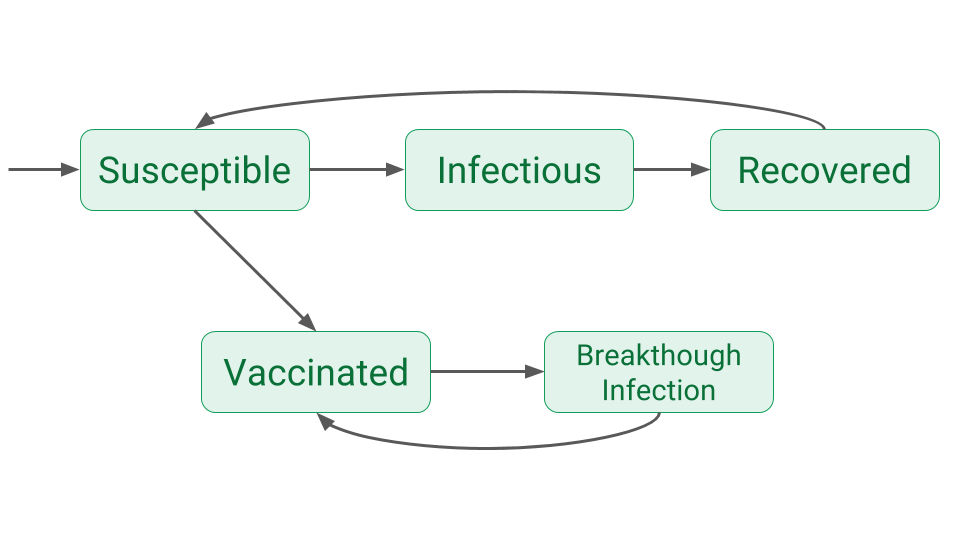
\includegraphics[trim={0 0 0 3cm}, clip,width=0.9\textwidth]{flow_diagram}
            \end{figure}
            \end{column}

      \end{block}
    \end{column}
    \begin{column}{\sepwid}\end{column}			% empty spacer column

    \begin{column}{0.9\onecolwid}
        \begin{block}{\textcolor{Black}{\Large{Results: Age Mixing Structures}}}
        		\begin{figure}
        		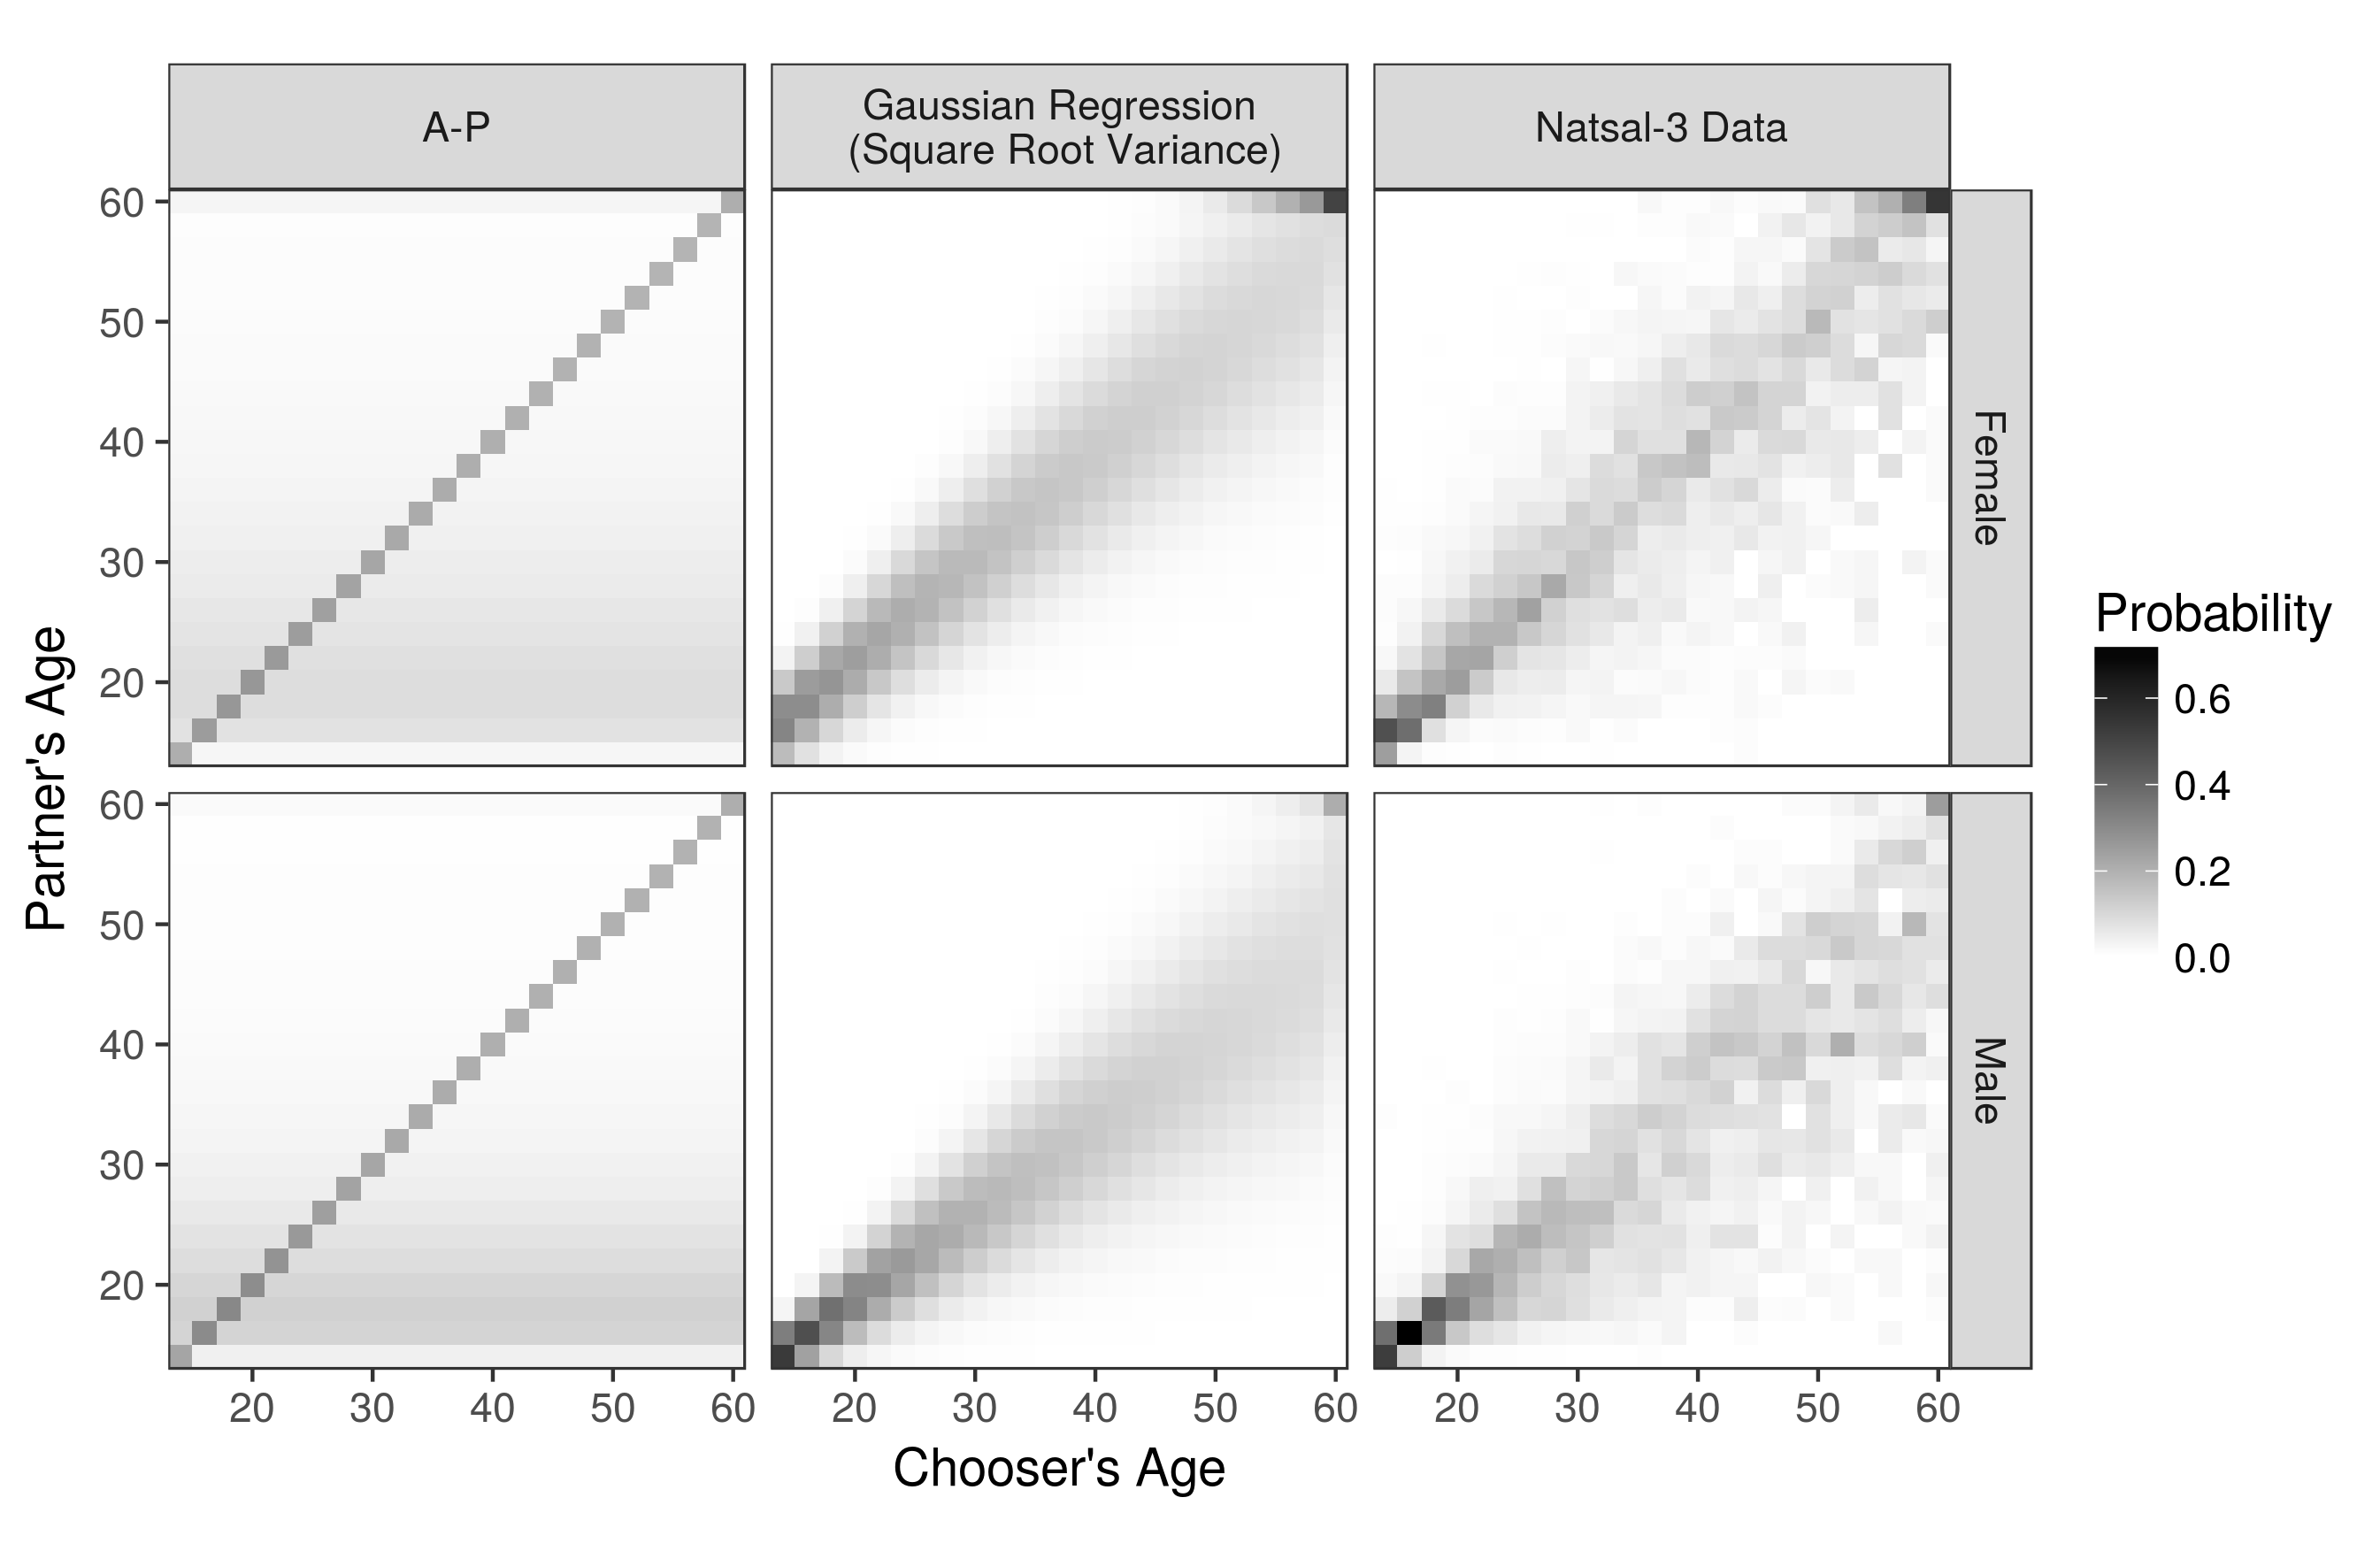
\includegraphics[width = \textwidth]{comparison_levelplots_normal_only}
        		\caption{From left to right: the A-P structure,
                    a regression model with Laplace distributed errors and
                    variance as a linear function of age, and the Natsal data. Note the constant probabilities
                    in rows of the A-P structure.}\label{fig:1}
        		\end{figure}
    \begin{figure}
        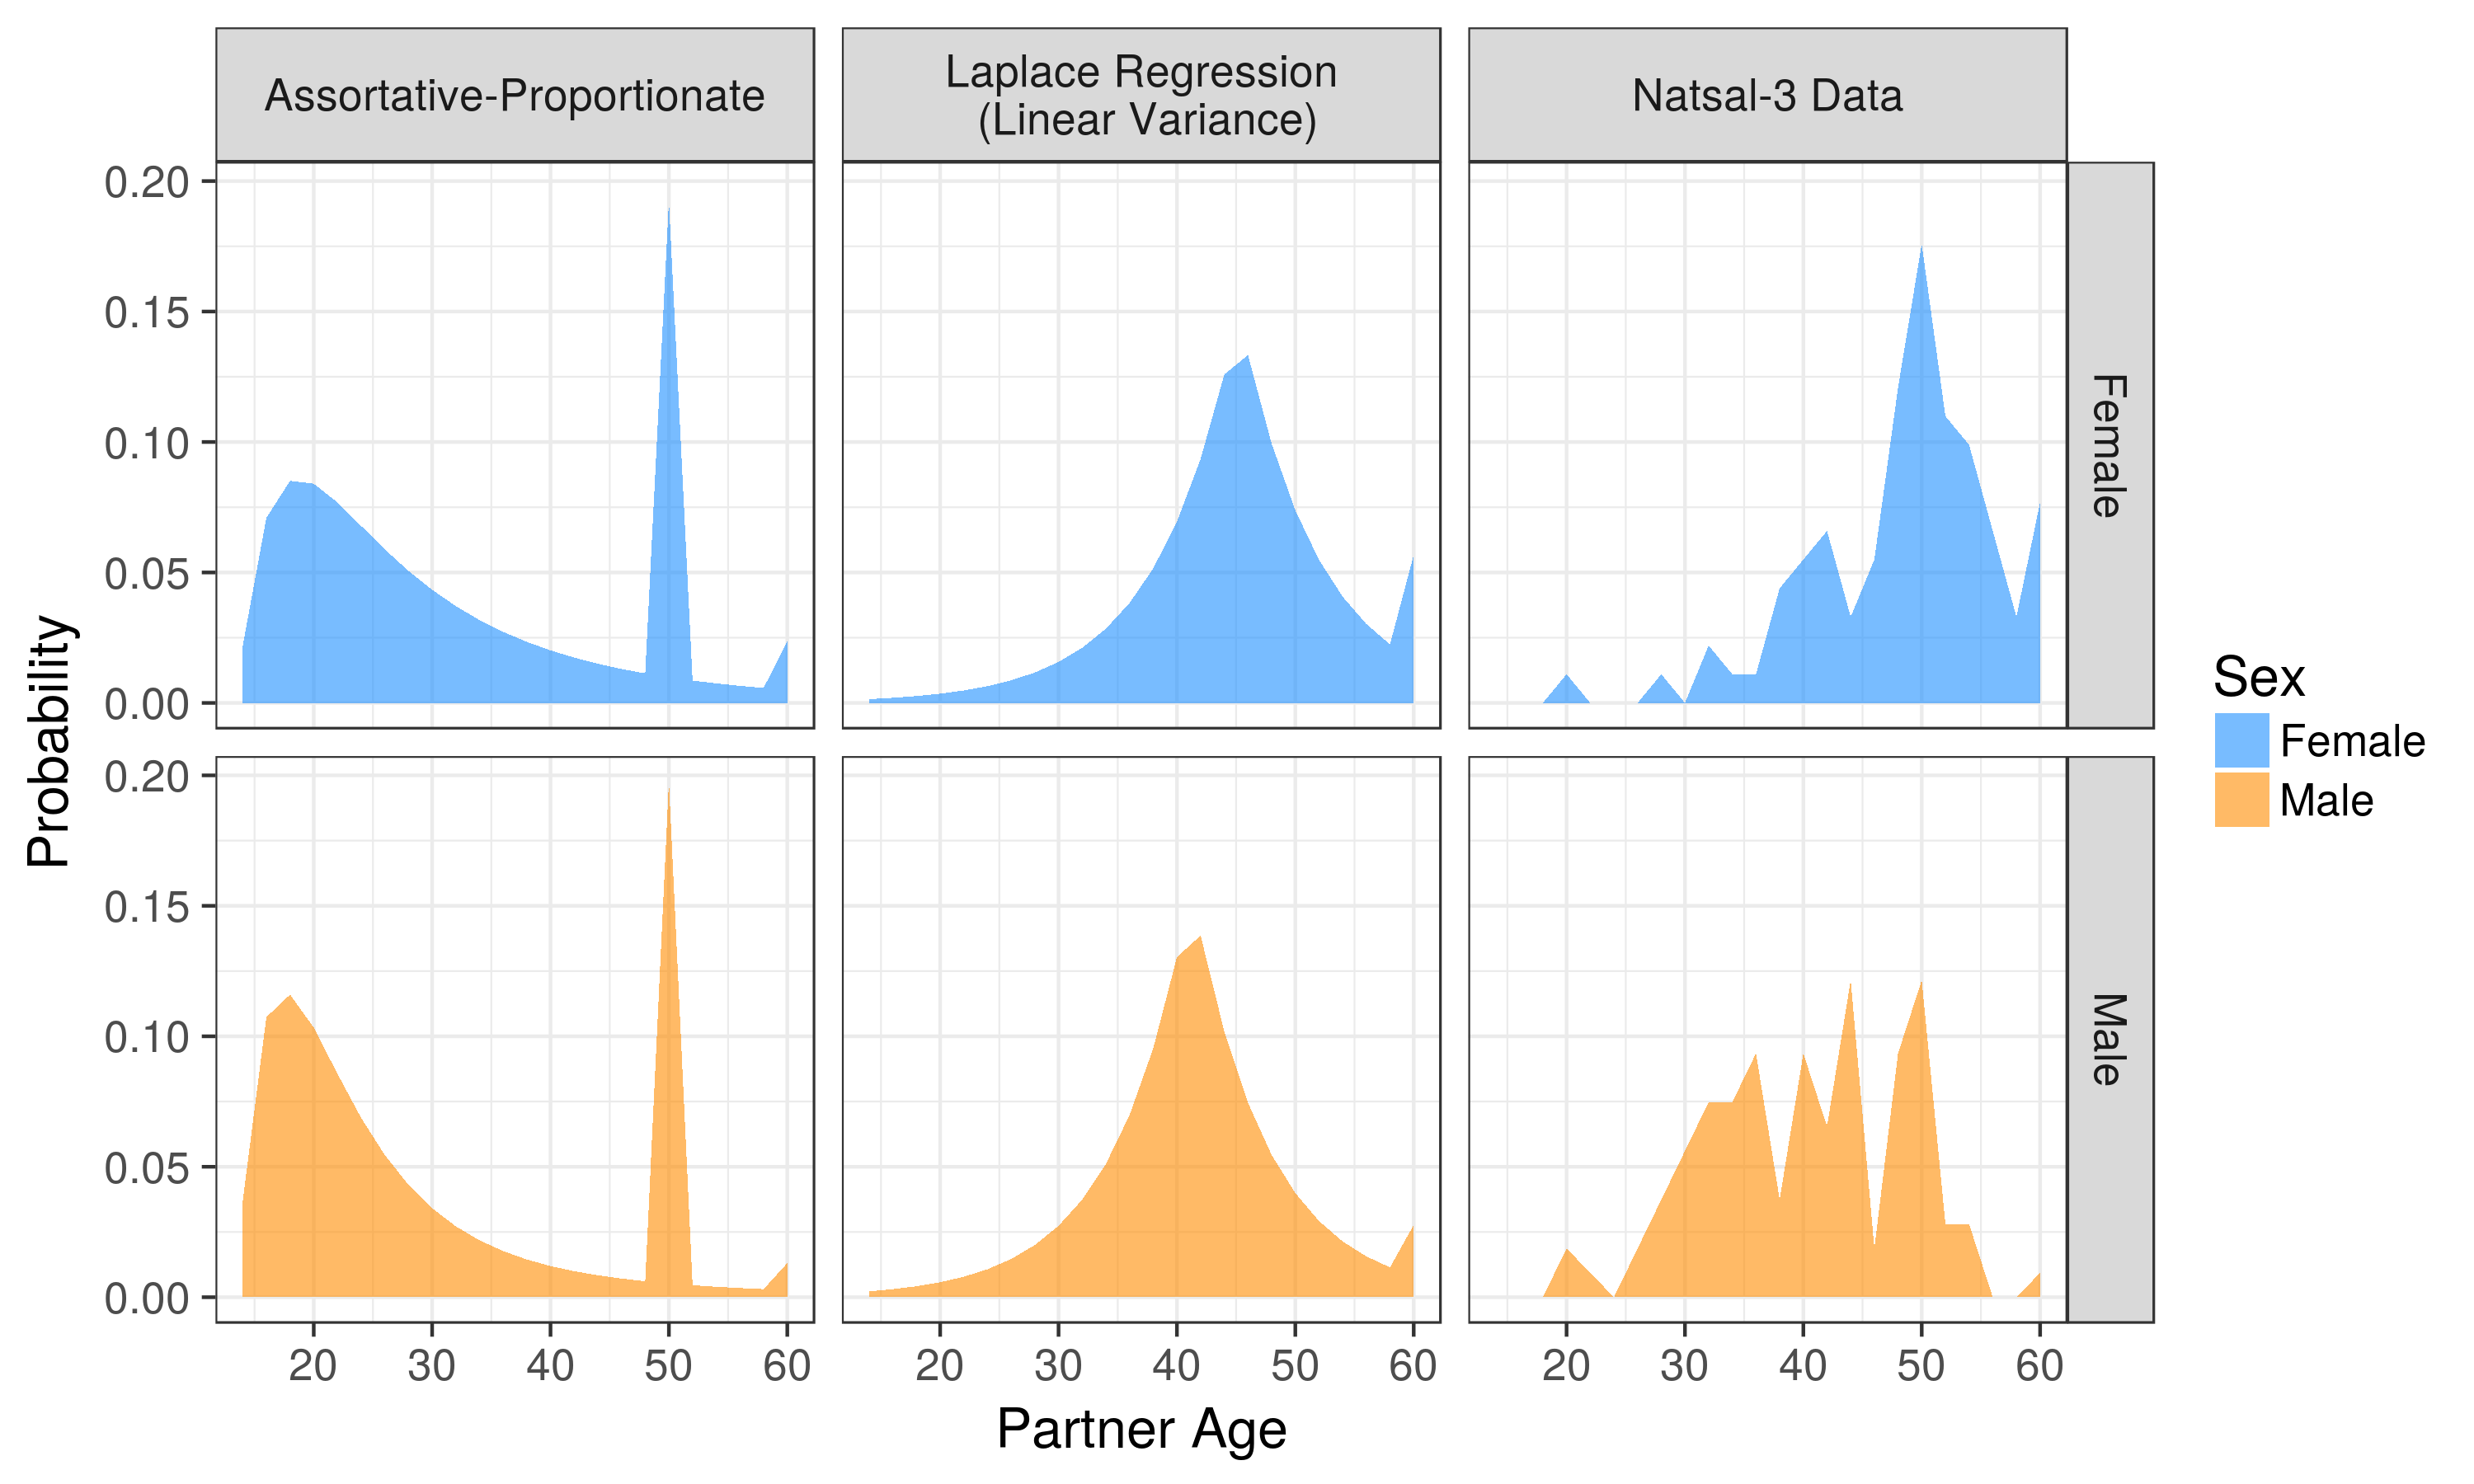
\includegraphics[width=0.8\textwidth]{comparison_age50}
        \caption{The partner age distributions for 50-year-old male and females.}
    \end{figure}
        \end{block}
      \vskip2ex
      \begin{block}{\textcolor{Black}{\Large{Results: Likelihood Comparison}}}
            \begin{figure}
                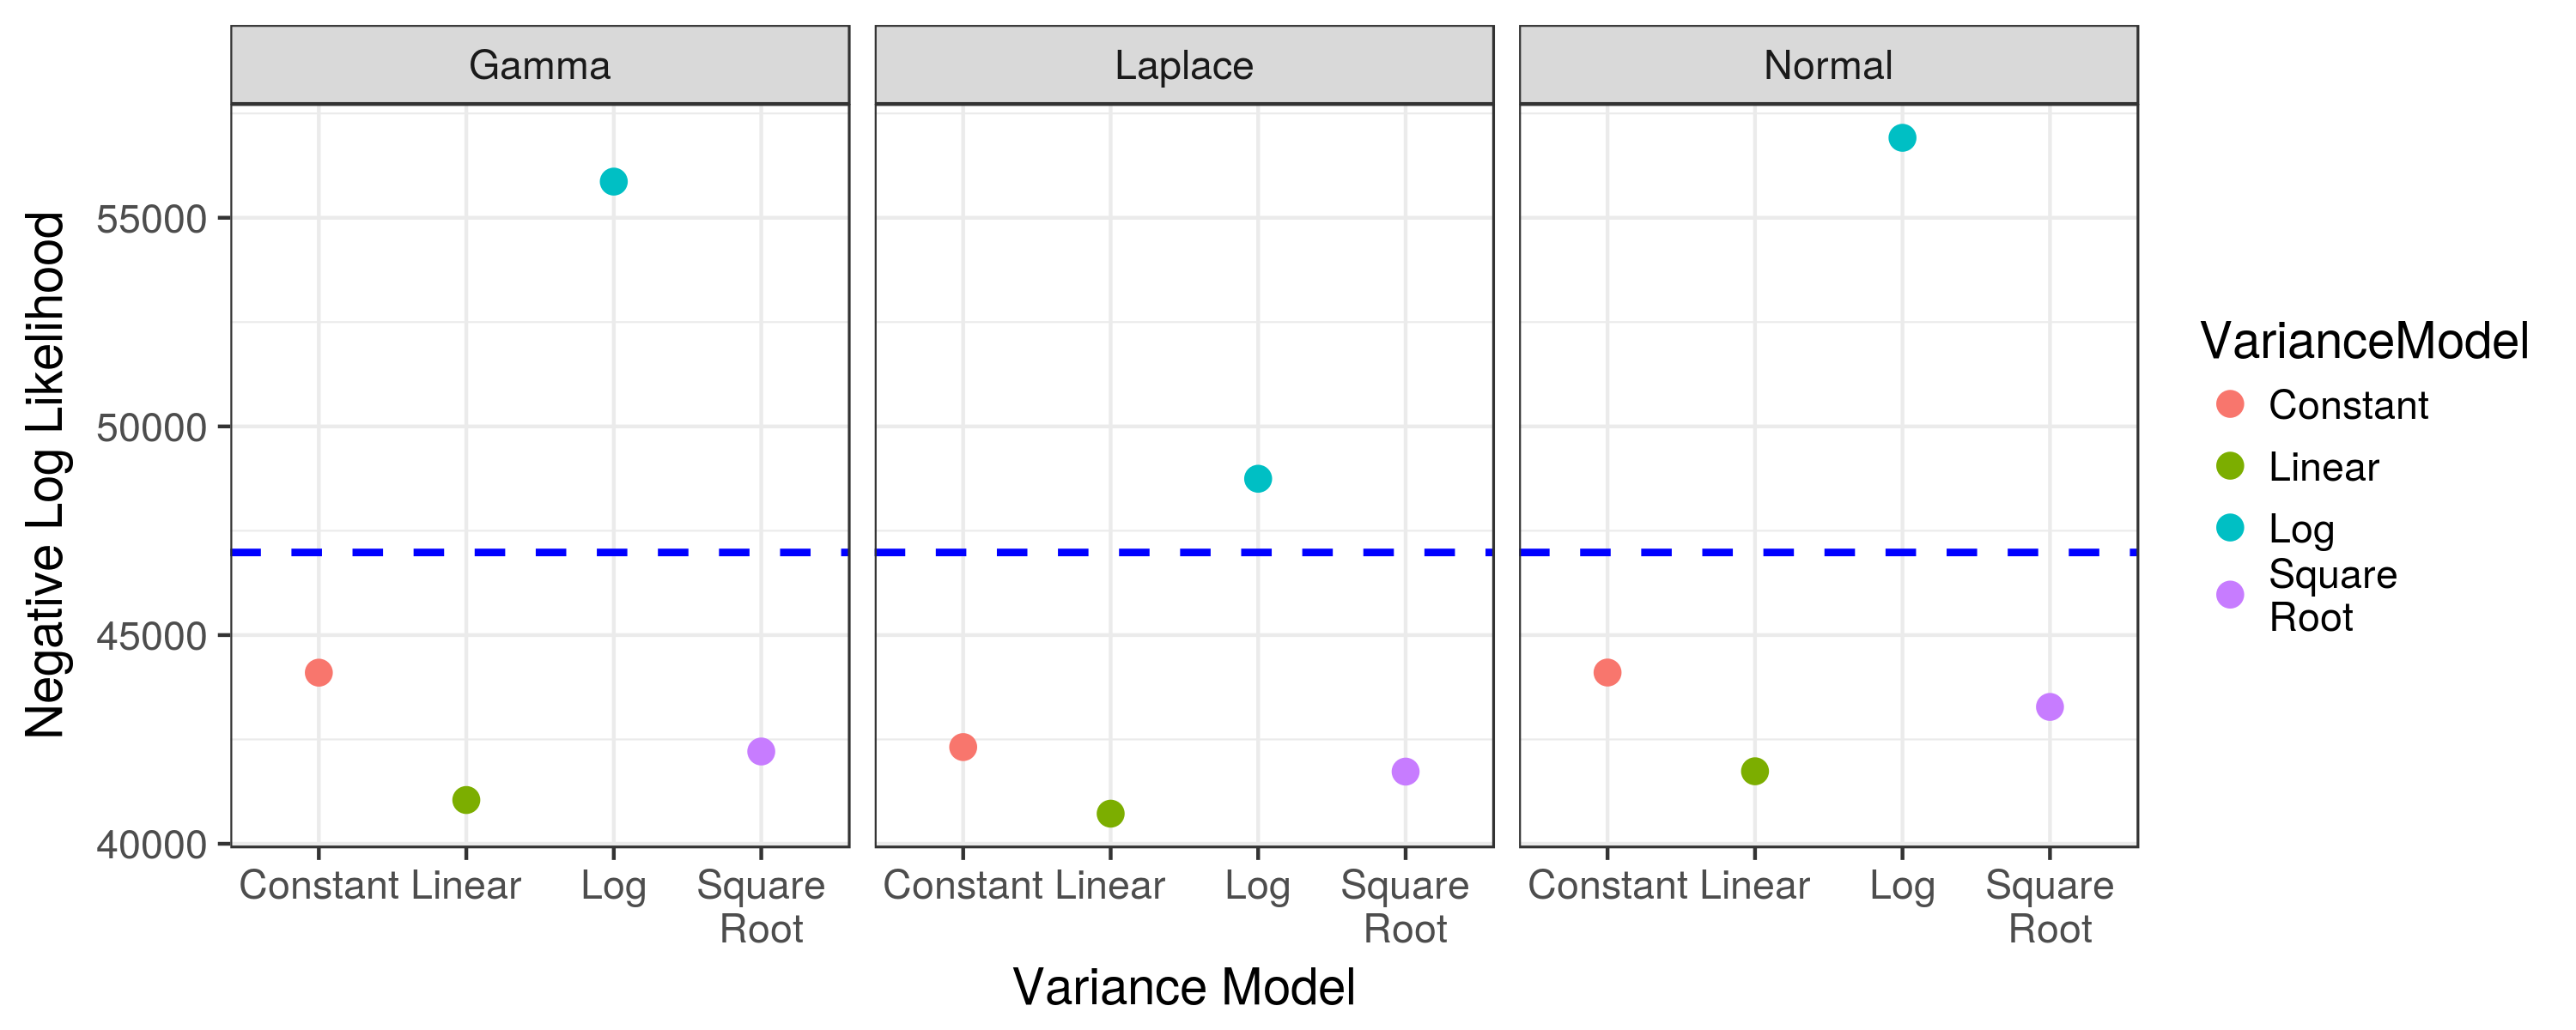
\includegraphics[width=\textwidth]{negLogLikelihoodAll}
                \caption{Likelihood of Natsal age mixing data under different mixing assumptions.
                The dotted blue line is the likelihood under A-P}\label{fig:2}
            \end{figure}
        \end{block}
\end{column}

\begin{column}{\sepwid}\end{column}

\begin{column}{\onecolwid}
      \begin{block}{\textcolor{Black}{\Large{Results: Extending
                Vaccination to 26-39-year-old Females}}}
            \begin{figure}
            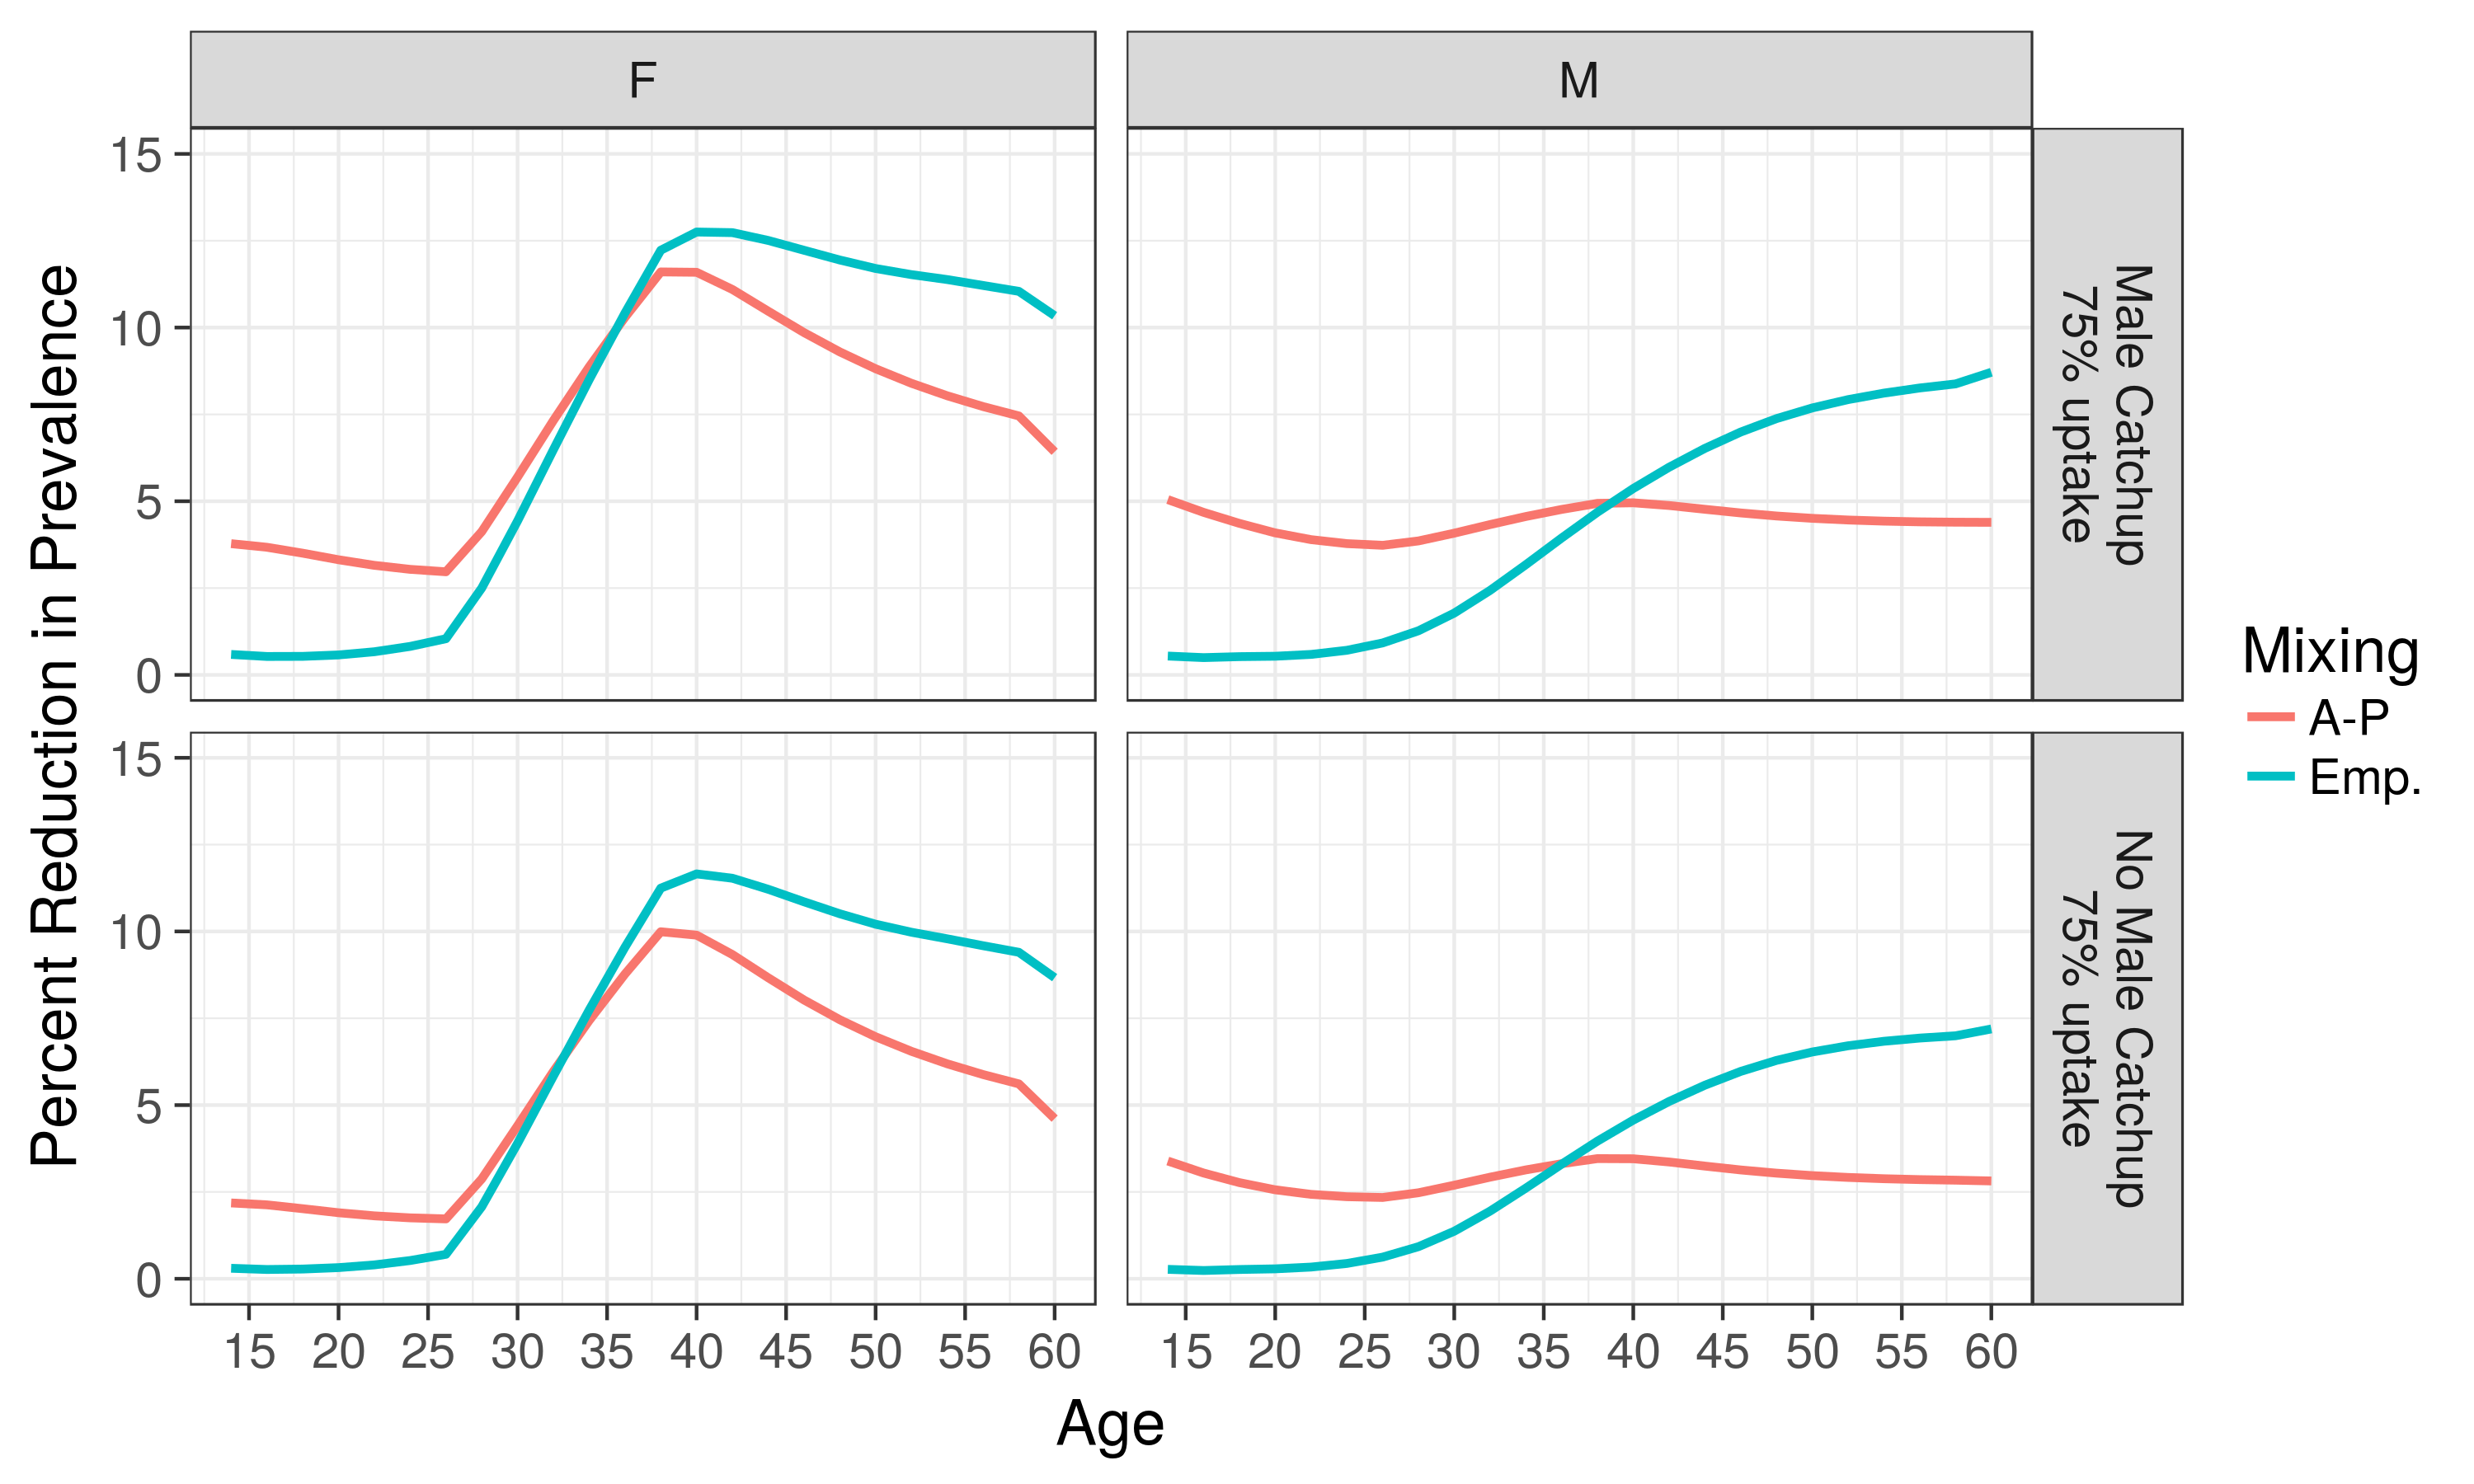
\includegraphics[width=0.8\textwidth]{relative_reduction_extending_coverage}
                \caption{Relative reduction in prevalence due to extending vaccination, by sex, age, and male catch-up scenario.}\label{fig:3}
            \end{figure}
      \end{block}
      \vskip2ex
    \begin{block}{Summary Measures}
        \begin{center}
            \begin{table}
                   \caption{Ratio of percentage reduction in
                    prevalence predicted by A-P model to that predicted by empirical model.
                   }
                \csvautobooktabularcenter{reduction_table.csv}
            \end{table}
        \end{center}
        \begin{itemize}
            \item The A-P model
                predicts a reduction in prevalence \textbf{7 times greater} (young males) and \textbf{5 times greater} (young females)
                than empirical model prediction.
            \item A-P model predicts slightly more than one
                half of the reduction for older males, and slightly
                less than 3/4 of the benefit for older females.
        \end{itemize}
    \end{block}
    \vskip2ex
    \begin{alertblock}{Conclusions}
        \begin{itemize}
            \item Standard regression models fit Natsal-3 age mixing data
                better than the A-P mixing structure.
            \item The A-P mixing structure overestimates the
                sexual connection between those above and below 30.
            \item The choice of mixing structure impacts model-estimated vaccine benefits.
            \item A model with an A-P mixing structure:
                \begin{itemize}
                    \item Overestimates reduction in HPV prevalence for younger individuals
                    \item Understimates reduction in prevalence for older individuals
                \end{itemize}
        \end{itemize}
    \end{alertblock}
%    \begin{block}{Limitations}
%        \begin{itemize}
%            \item Model was relatively simple.
%            \item We only consider heterosexual partnerships (like most HPV models).
%            \item Only use one survey to compare goodness of fit.
%        \end{itemize}
%    \end{block}
\vskip2ex
    \begin{block}{Future Directions}
        \begin{itemize}
            \item Analyze other sexual behavior surveys
                (National Survey of Family Growth, etc.) and compare results.
            \item Extend HPV  model to include cervical cancer and other outcomes, for cost-effectiveness analysis.
            \item Calibrate model to HPV prevalence and incidence
                and examine degree to which calibration corrects for mixing structure differences.
            \item Develop empirical mixing estimates for non-heterosexual sexual mixing.
        \end{itemize}
    \end{block}
%    \begin{block}{Acknowledgements}
%		This work was supported by the Howard Hughes Medical Institute Off-Campus Data Scientist Fellowship.
%	\end{block}
%    \begin{block}{References}
%	  \begin{footnotesize}
%	  \printbibliography
%	  \end{footnotesize}
%	\end{block}
\end{column}
\begin{column}{\sepwid}\end{column}			% empty spacer column

\end{columns}
\end{frame}
\end{document}
